\documentclass{article}
%\usepackage{mathpazo}
\usepackage{lmodern}
\usepackage{amsmath}
\usepackage{graphicx}

\title{SHG yield in MKS: a complete derivationb}

\begin{document}
We follow the derivation established in Ref. \cite{mendozaEPI04}.

\section{SHG yield in CGS}

We define the radiated SHG yied as 

\begin{equation*}
R(\omega) = \frac{I(2\omega)}{I^{2}(\omega)},
\end{equation*}
with the intensity as\footnote{The original derivation, and Ref. \cite{reiningPRB94} state the intensity has a factor of $c/8\pi$.}
\begin{equation*}
I(\omega) = \frac{c}{2\pi}\vert E(\omega)\vert^{2},
\end{equation*}
so,
\begin{equation}\label{final}
R(\omega) = \frac{\frac{c}{2\pi}\vert E(2\omega)\vert^{2}}{(\frac{c}{2\pi})^{2}\vert E(\omega)\vert^{4}} = \frac{2\pi}{c}\frac{\vert E(2\omega)\vert^{2}}{\vert E(\omega)\vert^{4}}.
\end{equation}

We start from the derivation in Ref. \cite{mizrahiJOSA88}. See Fig. \ref{3layers}. The electric field radiated by a polarized sheet is
\begin{align}
E_{p\pm} &= \frac{2\pi i\omega}{c k_{z}}\hat{\mathbf{p}}_{\pm}\cdot\boldsymbol{\mathcal{P}},\label{eq:ep_miz}\\
E_{s} & = \frac{2\pi i\omega}{c k_{z}}\hat{\mathbf{s}}\cdot\boldsymbol{\mathcal{P}}\label{eq:es_miz},
\end{align}
where,
\begin{equation}
k_{z} = \sqrt{\epsilon(\omega) - \sin^{2}\theta},
\end{equation}
and the nonlinear polarization produced by the incoming fields is,
\begin{equation}
\mathcal{P}_{i}=\chi_{ijk}E_j(\omega)E_k(\omega),
\end{equation} 
where repeated indices are to be summed over. The unit vectors for the polarization in $s$ and $p$ directions are
\begin{align}
\hat{\mathbf{p}}_{\pm} &= \frac{1}{\sqrt{\epsilon}}(\mp k_{z}\hat{\mathbf{x}} - \sin\theta\hat{\mathbf{z}}),\label{eq:pvectors}\\
\hat{\mathbf{s}} &= \hat{\mathbf{y}}.\label{eq:svectors}
\end{align}

\begin{figure}[t]
\centering
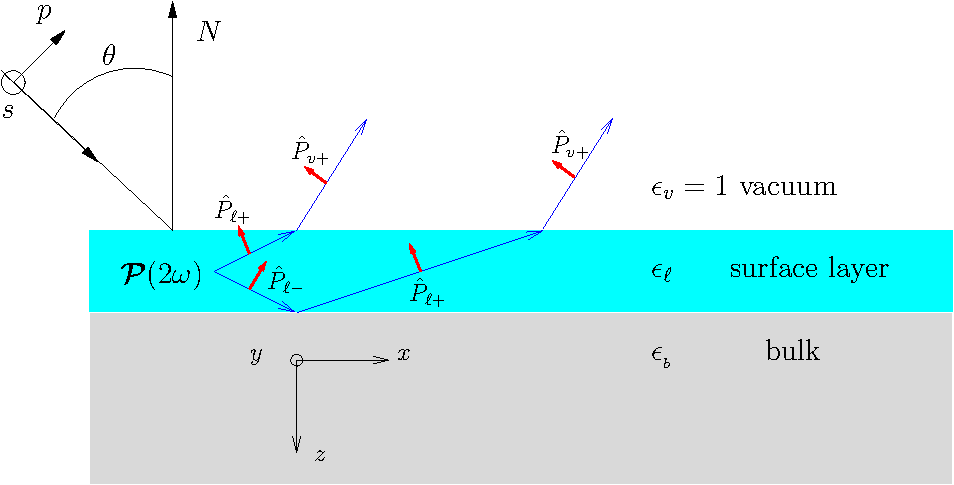
\includegraphics[width=0.7\textwidth]{plots/3layers}
\caption{Sketch of the three layer model for SHG. Vacuum is on top with
$\epsilon=1$, the layer with non-linear polarization
$\boldsymbol{\mathcal{P}}(2\omega)$ is characterized with
$\epsilon_{\ell(}\omega)$ and the bulk with $\epsilon_{b}(\omega)$. In the
dipolar approximation the bulk does not radiate SHG. The thin arrows are along
the direction of propagation, and the unit vectors for $p$-polarization are
denoted with thick arrows (capital letters denote SH components). The unit
vector for $s$-polarization points along $y$ (out of the page). $N$ is normal
to the surface, and $\theta$ is the angle of incidence for $p$ or $s$ input
polarization.\label{3layers}}
\end{figure}

We define the transmission, $\mathbf{T}$, and reflection, $\mathbf{R}$, tensors as,
\begin{equation}\label{r5}
\mathbf{T}_{\ell v}= \hat{\mathbf{s}}T_{s}^{\ell v}\hat{\mathbf{s}} + \hat{\mathbf{P}}_{v+}\tilde{T}_{p}^{\ell v} \hat{\mathbf{P}}_{\ell +},
\end{equation}
and
\begin{equation}\label{r6}
\mathbf{R}_{\ell b}= \hat{\mathbf{s}}R_{s}^{\ell b}\hat{\mathbf{s}} + \hat{\mathbf{P}}_{\ell +}R_{p}^{\ell b} \hat{\mathbf{P}}_{\ell -},
\end{equation}
where variables in capital letters are evaluated at the harmonic frequency
$2\omega$. Notice that since $\hat{\mathbf{s}}$ is independent of $\omega$, then
$\hat{\mathbf{s}}=\hat{\mathbf{s}}$. The Fresnel factors, $T_{i}$, $R_{i}$,
and $\tilde{T}_{p}$, for $i=s,p$ polarization, are evaluated at the appropriate
interface $\ell v$ or $\ell b$, and will be given below. The extra subscript
in $\hat{\mathbf{P}}$ denotes the corresponding dielectric function to be used in its
evaluation, i.e. $\epsilon_{v}=1$ for vacuum ($v$),
$\epsilon_{\ell}$ for the layer ($\ell$),
and $\epsilon_{b}$ for the bulk ($b$).
Therefore, the total radiated field at $2\omega$ is
\begin{align}\label{r7}
\mathbf{E}(2\omega) &=
E_{s}(2\omega)\left(\mathbf{T}_{\ell v} + \mathbf{T}_{\ell v}\cdot\mathbf{R}_{\ell b}\right)\cdot\hat{\mathbf{s}}\nonumber\\ 
&+ E_{p+}(2\omega)\mathbf{T}_{\ell v}\cdot\hat{\mathbf{P}}_{\ell +} + E_{p-}(2\omega)\mathbf{T}_{\ell v}\cdot\mathbf{R}_{\ell b}\cdot\hat{\mathbf{P}}_{\ell -}.
\end{align}
First, we develop an intermediate result,
\begin{align*}
\mathbf{T}_{\ell v}\cdot\mathbf{R}_{\ell b} &= (\hat{\mathbf{s}}T_{s}^{\ell v}\hat{\mathbf{s}} + \hat{\mathbf{P}}_{v+}\tilde{T}_{p}^{\ell v} \hat{\mathbf{P}}_{\ell +})\cdot(\hat{\mathbf{s}}R_{s}^{\ell b}\hat{\mathbf{s}} + \hat{\mathbf{P}}_{\ell +}R_{p}^{\ell b} \hat{\mathbf{P}}_{\ell -})\\
&= \hat{\mathbf{s}}T_{s}^{\ell v}R_{s}^{\ell b}\hat{\mathbf{s}} + \hat{\mathbf{P}}_{v+}\tilde{T}_{p}^{\ell v}R_{p}^{\ell b}\hat{\mathbf{P}}_{\ell -}
\end{align*}

We apply this result for the $E_{s}$ term in Eq. \eqref{r7},
\begin{align}\label{eq:es}
\left(\mathbf{T}_{\ell v} + \mathbf{T}_{\ell v}\cdot\mathbf{R}_{\ell b}\right)\cdot\hat{\mathbf{s}} = &\Bigl[\hat{\mathbf{s}}T_{s}^{\ell v}\hat{\mathbf{s}} + \hat{\mathbf{P}}_{v+}\tilde{T}_{p}^{\ell v} \hat{\mathbf{P}}_{\ell +}\nonumber\\
&+ \hat{\mathbf{s}}T_{s}^{\ell v}R_{s}^{\ell b}\hat{\mathbf{s}} + \hat{\mathbf{P}}_{v+}\tilde{T}_{p}^{\ell v}R_{p}^{\ell b}\hat{\mathbf{P}}_{\ell -} \Bigr]\cdot\hat{\mathbf{s}}\nonumber\\
= &\Bigl[\hat{\mathbf{s}}\tilde{T}_{s}^{\ell v}\bigl(1 + R_{s}^{\ell b})\hat{\mathbf{s}}\Bigr]\cdot\hat{\mathbf{s}}\nonumber\\
= &\hat{\mathbf{s}}\tilde{T}_{s}^{\ell v}\bigl(1 + R_{s}^{\ell b})
\end{align}
For $E_{p+}$,
\begin{align}\label{eq:ep+}
\mathbf{T}_{\ell v}\cdot\hat{\mathbf{P}}_{\ell +} &= (\hat{\mathbf{s}}T_{s}^{\ell v}\hat{\mathbf{s}} + \hat{\mathbf{P}}_{v+}\tilde{T}_{p}^{\ell v} \hat{\mathbf{P}}_{\ell +})\cdot\hat{\mathbf{P}}_{\ell +}\nonumber\\
&= \hat{\mathbf{P}}_{v+}\tilde{T}_{p}^{\ell v}
\end{align}
and lasty for For $E_{p-}$,
\begin{align}\label{eq:ep-}
\mathbf{T}_{\ell v}\cdot\mathbf{R}_{\ell b}\cdot\hat{\mathbf{P}}_{\ell -} &= (\hat{\mathbf{s}}T_{s}^{\ell v}R_{s}^{\ell b}\hat{\mathbf{s}} + \hat{\mathbf{P}}_{v+}\tilde{T}_{p}^{\ell v}R_{p}^{\ell b}\hat{\mathbf{P}}_{\ell -})\cdot\hat{\mathbf{P}}_{\ell -}\nonumber\\
&= \hat{\mathbf{P}}_{v+}\tilde{T}_{p}^{\ell v}R_{p}^{\ell b}
\end{align}
We replace Eqs. \eqref{eq:es}, \eqref{eq:ep+}, and \eqref{eq:ep-} into Eq. \eqref{r7},
\begin{align}\label{eq:e2w}
\mathbf{E}(2\omega) &=
E_{s}(2\omega)\Bigl[\hat{\mathbf{s}}\tilde{T}_{s}^{\ell v}\bigl(1 + R_{s}^{\ell b})\Bigr]\nonumber\\ 
&+ E_{p+}(2\omega)\Bigl[\hat{\mathbf{P}}_{v+}\tilde{T}_{p}^{\ell v}\Bigr] + E_{p-}(2\omega)\Bigl[\hat{\mathbf{P}}_{v+}\tilde{T}_{p}^{\ell v}R_{p}^{\ell b}\Bigr].
\end{align}

From Eqs. \eqref{eq:ep_miz} and \eqref{eq:es_miz}, we get that 
\begin{align}
E_{p\pm}(2\omega) &= \frac{4\pi i\omega}{c K_{z}}\hat{\mathbf{p}}_{\pm}\cdot\boldsymbol{\mathcal{P}},\label{eq:ep_miz2w}\\
E_{s}(2\omega) & = \frac{4\pi i\omega}{c K_{z}}\hat{\mathbf{s}}\cdot\boldsymbol{\mathcal{P}}\label{eq:es_miz2w},
\end{align}

Combining Eqs. \eqref{eq:ep_miz2w} and \eqref{eq:es_miz2w} into Eq. \eqref{eq:e2w}
\begin{align}
\mathbf{E}(2\omega) &= \frac{4\pi i\omega}{c K_{z}}\Bigl[\hat{\mathbf{s}}\tilde{T}_{s}^{\ell v}\bigl(1 + R_{s}^{\ell b})\hat{\mathbf{s}} + \hat{\mathbf{P}}_{v+}\tilde{T}_{p}^{\ell v}\hat{\mathbf{P}}_{\ell +} + \hat{\mathbf{P}}_{v+}\tilde{T}_{p}^{\ell v}R_{p}^{\ell b}\hat{\mathbf{P}}_{\ell -}\Bigr]\cdot\boldsymbol{\mathcal{P}}\\
&= \frac{4\pi i\omega}{c K_{z}}\Bigl[\hat{\mathbf{s}}\tilde{T}_{s}^{\ell v}\bigl(1 + R_{s}^{\ell b})\hat{\mathbf{s}} + \hat{\mathbf{P}}_{v+}\tilde{T}_{p}^{\ell v}\bigl(\hat{\mathbf{P}}_{\ell +} + R_{p}^{\ell b}\hat{\mathbf{P}}_{\ell -}\bigr)\Bigr]\cdot\boldsymbol{\mathcal{P}}\\
&= \frac{4\pi i\omega}{c K_{z}}\mathbf{H}\cdot\boldsymbol{\mathcal{P}}
\end{align}
which matches Eq. (31) from Ref. \cite{mendozaEPI04}. We establish some simple relationships between $T$ and $R$,
\begin{align}\label{r11}
T_{s}^{\ell v} &= \frac{K_{z\ell}}{\cos\theta}\,T_{s}^{v\ell},  \quad\quad
\tilde{T}_p^{\ell v} = \frac{\sqrt{\epsilon_{\ell}(2\omega)}K_{z\ell}}{\cos\theta}\,T^{v\ell}_{p},\\
1 - R^{\ell b}_{p} &= \frac{\epsilon_{\ell}(2\omega)K_{zb}}{K_{z\ell}}\,T_{p}^{\ell b}, \quad\quad 
1 + R_{p}^{\ell b} = \epsilon_{b}(2\omega)T_{p}^{\ell b},\label{r11d}
\end{align}

The magnitude of the radiated field is given by
$E(2\omega)=\hat{\mathbf{e}}^{out}\cdot\mathbf{E}(2\omega)$,
where $\hat{\mathbf{e}}^{out}$ is the polarization vector of the radiated field, for
instance $\hat{\mathbf{s}}$ or $\hat{\mathbf{P}}_{v+}$. Then we write
\begin{equation}\label{r10}
E(2\omega)=\frac{4\pi i\omega}{c}\mathbf{e}^{\,2\omega}\cdot\boldsymbol{\mathcal{P}},
\end{equation}
so
\begin{equation}
\mathbf{e}^{\,2\omega} = \frac{1}{K_{z\ell}}\hat{\mathbf{e}}^{out}\cdot\mathbf{H}
\end{equation}

We rewrite $\mathbf{H}$ using Eqs. \eqref{r11}, \eqref{r11d}, \eqref{eq:pvectors}, and \eqref{eq:svectors},
\begin{equation}
\mathbf{H} = \frac{K_{zl}}{\cos\theta}\left[\hat{\mathbf{s}}T_{s}^{v\ell}T_{s}^{\ell b}\hat{\mathbf{y}} - \hat{\mathbf{P}}_{v+}T_{p}^{v\ell}T_{p}^{\ell b}\bigl(\epsilon_{\ell}(2\omega)K_{zb}\hat{\mathbf{x}} + \epsilon_{b}(2\omega)\sin\theta\hat{\mathbf{z}}\bigr)\right],
\end{equation}
and so,
\begin{equation}
\mathbf{e}^{\,2\omega} = \frac{1}{\cos\theta}\hat{\mathbf{e}}^{out}\cdot\left[\hat{\mathbf{s}}T_{s}^{v\ell}T_{s}^{\ell b}\hat{\mathbf{y}} - \hat{\mathbf{P}}_{v+}T_{p}^{v\ell}T_{p}^{\ell b}\bigl(\epsilon_{\ell}(2\omega)K_{zb}\hat{\mathbf{x}} + \epsilon_{b}(2\omega)\sin\theta\hat{\mathbf{z}}\bigr)\right]
\end{equation}

We can now write our $2\omega$ radiated fields as,
\begin{align}
E_{s}(2\omega) &= \frac{4\pi i \omega}{c\cos\theta}\Bigl[T_{s}^{v\ell}T_{s}^{\ell b}\hat{\mathbf{y}}\Bigr]\cdot\boldsymbol{\mathcal{P}} = \frac{4\pi i \omega}{c\cos\theta}T_{s}^{v\ell}T_{s}^{\ell b}\chi_{yij}E_{i}(\omega)E_{j}(\omega),\label{eq:es2w}\\
E_{p}(2\omega) &= -\frac{4\pi i \omega}{c\cos\theta}T_{p}^{v\ell}T_{p}^{\ell b}\Bigl[\epsilon_{\ell}(2\omega)K_{zb}\hat{\mathbf{x}} + \epsilon_{b}(2\omega)\sin\theta\hat{\mathbf{z}}\Bigr]\cdot\boldsymbol{\mathcal{P}}\nonumber\\
&= -\frac{4\pi i \omega}{c\cos\theta}T_{p}^{v\ell}T_{p}^{\ell b}\Bigl[\epsilon_{\ell}(2\omega)K_{zb}\chi_{xij} + \epsilon_{b}(2\omega)\sin\theta\chi_{zij}\Bigr]E_{i}(\omega)E_{j}(\omega).\label{eq:ep2w}
\end{align}

As mentioned before $E_{i}(\omega)$ is the incident field given by the external
field properly screened; then we have
\begin{equation}\label{r15}
\mathbf{E}_{s}(\omega)=E_{o} t_{s}^{v\ell}\left(1 + r_{s}^{\ell b}\right)\hat{\mathbf{y}},
\end{equation}
and
\begin{equation}\label{r16}
\mathbf{E}_{p}(\omega)=E_{o}\left[
\tilde{t}_p^{v\ell}\left(1-r_p^{\ell b}\right)\cos\theta_\ell\hat{\mathbf{x}}
-\tilde{t}_p^{v\ell}\left(1+r_p^{\ell
b}\right)\sin\theta_\ell\hat{\mathbf{z}}\right],
 \end{equation}
where $E_{o}$ is the incoming amplitude and $\theta_\ell$ is the angle of
refraction in the layer. Notice that the transmitted and reflected fields in
the layer are taken into $\mathbf{E}_{s}$ and $\mathbf{E}_{p}$. From Eqs.
(\ref{r11}-\ref{r11d}) we get
\begin{equation}\label{r17}
\mathbf{E}_{s}(\omega)=E_{o} t_s^{v\ell}t_s^{\ell b}\hat{\mathbf{y}},
\end{equation}
and
\begin{equation}\label{r18}
\mathbf{E}_{p}(\omega)=E_{o} t_p^{v\ell}t_p^{\ell b}\left(\epsilon_{\ell}(\omega)k_{zb}\hat{\mathbf{x}} - \epsilon_{b}(\omega)\sin\theta\hat{\mathbf{z}}\right).
\end{equation}

Substituting Eqs. \eqref{r17} and \eqref{r18} into Eqs. \eqref{eq:es2w} and \eqref{eq:ep2w}, then finally substituting those into Eq. \eqref{final}, we get

\begin{equation}\label{r19}
 R_{iF}=\frac{32\pi^3\omega^2}{(n_oe)^2c^3\cos^2\theta}
\left|T_F^{v\ell}T_F^{\ell b}(t_i^{v\ell}t_i^{\ell b})^2\,r_{iF}\right|^2,
\end{equation}
where $i$ (lower case) stands for initial polarization and $F$ (upper case)
stands for final polarization, with
\begin{equation}\label{r20}
r_{iP}=\left(\epsilon_\ell(2\omega)K_{zb}\chi_{xjk} + \epsilon_b(2\omega)\sin\theta\chi_{zjk}\right)
E_j^i E_k^i,
\end{equation}
and
\begin{equation}\label{r21}
r_{iS}=\chi_{yjk}  E_j^i E_k^i,
\end{equation}
where from Eqs. (\ref{r17}-\ref{r18}),
\begin{subequations}\label{r23}
\begin{align}
\mathbf{E}^s&=\hat{\mathbf{y}}\\
\mathbf{E}^p&=\epsilon_\ell(\omega)k_{zb}\hat{\mathbf{x}}-\epsilon_b(\omega)\sin\theta\hat{\mathbf{z}}.
\end{align}
\end{subequations}
The $n_oe$ factor in Eq. (\ref{r19}), with $n_o$ the electronic density,
renders $\boldsymbol{\chi}$ dimensionless.
To complete the required formulas, we write down the Fresnel factors,
\begin{equation}\label{e.f1}
t_s^{v\ell}=\frac{2\cos\theta}{\cos\theta+k_{z\ell}},
\quad\quad
t_p^{v\ell}=\frac{2\cos\theta}{\epsilon_\ell(\omega)\cos\theta+k_{z\ell}},
\end{equation}
\begin{equation}\label{e.f3}
t_s^{\ell b}=\frac{2k_{z\ell}}{k_{z\ell}+k_{zb}},
\quad\quad
t_p^{\ell b}=\frac{2k_{z\ell}}{\epsilon_b(\omega)k_{z\ell}+\epsilon_s(\omega)k_{zb}},
\end{equation}
where the appropriate term $\sqrt{\epsilon(\omega)}$ from the usual definition of
$t_p$ has been taken out to give Eqs. (\ref{r20}) and
(\ref{r21}).

\bibliographystyle{plain}
\bibliography{ref}

\end{document}
